\chapter{Technical Implementation and AI Integration}

\section{BCD.NET Platform Architecture}

\subsection{Platform Overview}
The BCD.NET platform represents a comprehensive digital transformation of BCD's networking capabilities, designed to enhance member engagement, facilitate deal flow, and provide intelligent matching services. The platform integrates modern web technologies with AI-powered features to create a seamless networking experience, building on the frameworks outlined in \citep{venugopal_containerized_microservices_architecture}.

\begin{figure}[h]
\centering
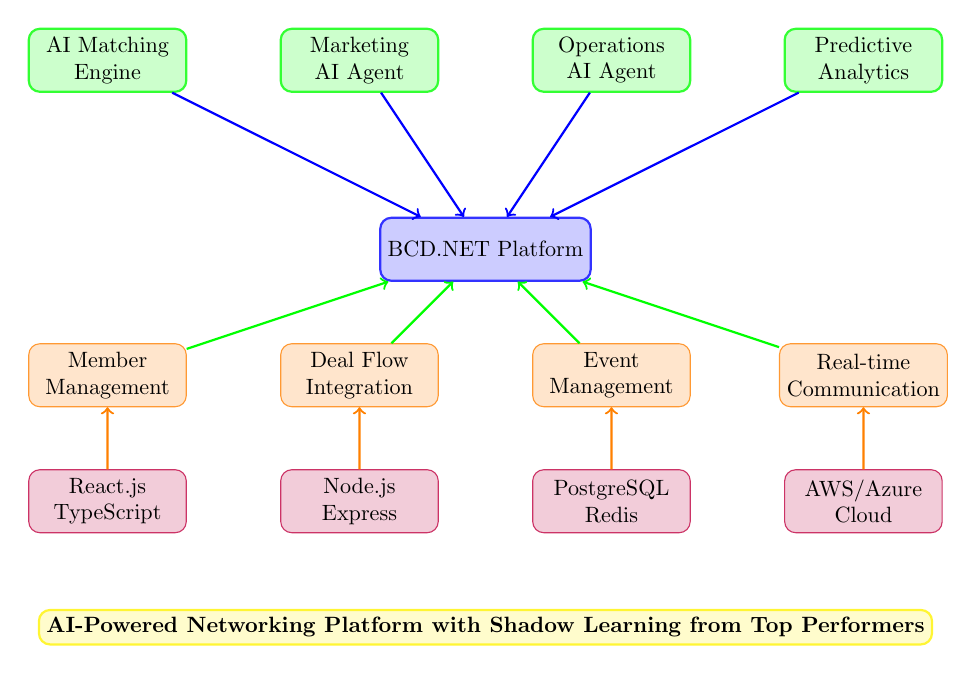
\begin{tikzpicture}[
    scale=0.8,
    transform shape,
    box/.style={rectangle, draw, rounded corners, minimum width=2.5cm, minimum height=1cm, align=center},
    platform/.style={box, fill=blue!20, draw=blue!80, thick},
    ai/.style={box, fill=green!20, draw=green!80, thick},
    feature/.style={box, fill=orange!20, draw=orange!80},
    tech/.style={box, fill=purple!20, draw=purple!80},
    arrow/.style={->, thick}
]

% Core Platform
\node[platform] (bcd) at (0,0) {BCD.NET Platform};

% AI Components
\node[ai] (matching) at (-6,3) {AI Matching\\Engine};
\node[ai] (marketing) at (-2,3) {Marketing\\AI Agent};
\node[ai] (operations) at (2,3) {Operations\\AI Agent};
\node[ai] (analytics) at (6,3) {Predictive\\Analytics};

% Core Features
\node[feature] (members) at (-6,-2) {Member\\Management};
\node[feature] (deals) at (-2,-2) {Deal Flow\\Integration};
\node[feature] (events) at (2,-2) {Event\\Management};
\node[feature] (communication) at (6,-2) {Real-time\\Communication};

% Technology Stack
\node[tech] (frontend) at (-6,-4) {React.js\\TypeScript};
\node[tech] (backend) at (-2,-4) {Node.js\\Express};
\node[tech] (database) at (2,-4) {PostgreSQL\\Redis};
\node[tech] (cloud) at (6,-4) {AWS/Azure\\Cloud};

% Connections
\draw[arrow, blue] (matching) -- (bcd);
\draw[arrow, blue] (marketing) -- (bcd);
\draw[arrow, blue] (operations) -- (bcd);
\draw[arrow, blue] (analytics) -- (bcd);

\draw[arrow, green] (members) -- (bcd);
\draw[arrow, green] (deals) -- (bcd);
\draw[arrow, green] (events) -- (bcd);
\draw[arrow, green] (communication) -- (bcd);

\draw[arrow, orange] (frontend) -- (members);
\draw[arrow, orange] (backend) -- (deals);
\draw[arrow, orange] (database) -- (events);
\draw[arrow, orange] (cloud) -- (communication);

% Platform highlights
\node[fill=yellow!20, draw=yellow!80, thick, rounded corners] at (0,-6) 
    {\textbf{AI-Powered Networking Platform with Shadow Learning from Top Performers}};

\end{tikzpicture}
\caption{BCD.NET Platform Architecture and AI Integration}
\label{fig:bcd-platform-architecture}
\end{figure}

\subsection{Technical Architecture}
\begin{itemize}
    \item \textbf{Frontend}: React.js with TypeScript for robust user interface
    \item \textbf{Backend}: Node.js with Express.js for scalable API development
    \item \textbf{Database}: PostgreSQL for relational data with Redis for caching
    \item \textbf{Authentication}: JWT-based secure authentication system
    \item \textbf{Real-time Communication}: WebSocket integration for instant messaging
    \item \textbf{Cloud Infrastructure}: AWS or Azure for scalable deployment
\end{itemize}

This architecture is informed by research from \citep{reiff_multiagent_sophisticated_system} and \citep{ferede_artificial_intelligence_ai}, which examine effective AI integration in modern software platforms.

\subsection{Core Platform Features}
\subsubsection{Member Management System}
\begin{itemize}
    \item Comprehensive member profiles with verification processes
    \item Advanced search and filtering capabilities
    \item Privacy controls and data protection compliance
    \item Integration with existing WhatsApp community
    \item Member activity tracking and engagement analytics
\end{itemize}

\subsubsection{Deal Flow Integration}
\begin{itemize}
    \item Deal posting and discovery system
    \item Investment opportunity matching
    \item Due diligence document sharing
    \item Deal tracking and status updates
    \item Investment syndicate formation tools
\end{itemize}

\subsubsection{Event Management}
\begin{itemize}
    \item Event creation and registration system
    \item Calendar integration and notifications
    \item Attendee management and networking facilitation
    \item Virtual and hybrid event capabilities
    \item Post-event analytics and feedback collection
\end{itemize}

\section{AI-Powered Platform Intelligence}

\subsection{Multi-Agent AI System Architecture}

The BCD.NET platform employs a sophisticated multi-agent AI system that provides intelligent automation and optimization across all platform functions, as documented in \:

\subsubsection{Core AI Agents}

\begin{itemize}
    \item \textbf{Member Matching Agent}: AI-powered member matching based on complementary skills, interests, and goals
    \item \textbf{Deal Flow Intelligence Agent}: Intelligent deal sourcing, qualification, and matching with member preferences
    \item \textbf{Event Optimization Agent}: AI-optimized event planning, attendance prediction, and networking facilitation
    \item \textbf{Content Intelligence Agent}: Personalized content delivery and knowledge sharing optimization
    \item \textbf{Network Health Agent}: Continuous monitoring of community engagement and satisfaction
\end{itemize}

\subsubsection{AI-Powered Features}

\begin{itemize}
    \item \textbf{Intelligent Member Onboarding}: AI-personalized onboarding experiences based on member background
    \item \textbf{Predictive Analytics}: Advanced forecasting of member behavior, deal flow trends, and platform growth
    \item \textbf{Real-Time Optimization}: Continuous platform optimization based on user behavior and feedback
    \item \textbf{Automated Content Generation}: AI-generated content for member communications and marketing
    \item \textbf{Intelligent Search and Discovery}: Advanced search algorithms for members, deals, and opportunities
\end{itemize}

\section{Detailed Development Architecture}

\subsection{Microservices Architecture Design}

The BCD.NET platform implements a sophisticated microservices architecture with clear separation of concerns and independent scalability, as documented in \citep{venugopal_containerized_microservices_architecture}.

\begin{figure}[h]
\centering
\begin{tikzpicture}[
    scale=0.6,
    transform shape,
    service/.style={rectangle, draw, rounded corners, minimum width=2.5cm, minimum height=1.2cm, align=center},
    api/.style={service, fill=blue!20, draw=blue!80, thick},
    core/.style={service, fill=green!20, draw=green!80},
    ai/.style={service, fill=orange!20, draw=orange!80, thick},
    data/.style={service, fill=purple!20, draw=purple!80},
    infra/.style={service, fill=red!20, draw=red!80},
    arrow/.style={->, thick},
    db/.style={cylinder, draw, minimum width=1.5cm, minimum height=1cm}
]

% API Gateway Layer
\node[api] (gateway) at (0,8) {API Gateway\\Kong/Envoy};

% Core Services
\node[core] (auth) at (-12,6) {Authentication\\Service};
\node[core] (user) at (-9,6) {User Management\\Service};
\node[core] (profile) at (-6,6) {Profile\\Service};
\node[core] (event) at (-3,6) {Event\\Service};
\node[core] (deal) at (0,6) {Deal Flow\\Service};
\node[core] (communication) at (3,6) {Communication\\Service};
\node[core] (notification) at (6,6) {Notification\\Service};
\node[core] (analytics) at (9,6) {Analytics\\Service};

% AI Services
\node[ai] (matching_ai) at (-12,4) {Matching\\AI Agent};
\node[ai] (marketing_ai) at (-9,4) {Marketing\\AI Agent};
\node[ai] (operations_ai) at (-6,4) {Operations\\AI Agent};
\node[ai] (content_ai) at (-3,4) {Content\\AI Agent};
\node[ai] (security_ai) at (0,4) {Security\\AI Agent};
\node[ai] (prediction_ai) at (3,4) {Prediction\\AI Agent};
\node[ai] (recommendation_ai) at (6,4) {Recommendation\\AI Agent};
\node[ai] (nlp_ai) at (9,4) {NLP\\AI Agent};

% Data Services
\node[data] (data_pipeline) at (-12,2) {Data\\Pipeline};
\node[data] (ml_pipeline) at (-9,2) {ML\\Pipeline};
\node[data] (feature_store) at (-6,2) {Feature\\Store};
\node[data] (model_registry) at (-3,2) {Model\\Registry};
\node[data] (data_lake) at (0,2) {Data\\Lake};
\node[data] (cache) at (3,2) {Cache\\Service};
\node[data] (search) at (6,2) {Search\\Engine};
\node[data] (monitoring) at (9,2) {Monitoring\\Service};

% Infrastructure
\node[infra] (load_balancer) at (-12,0) {Load\\Balancer};
\node[infra] (service_mesh) at (-9,0) {Service\\Mesh};
\node[infra] (message_queue) at (-6,0) {Message\\Queue};
\node[infra] (config) at (-3,0) {Config\\Service};
\node[infra] (discovery) at (0,0) {Service\\Discovery};
\node[infra] (circuit_breaker) at (3,0) {Circuit\\Breaker};
\node[infra] (rate_limiter) at (6,0) {Rate\\Limiter};
\node[infra] (monitoring) at (9,0) {Infrastructure\\Monitoring};

% Databases
\node[db] (postgres) at (-12,-2) {PostgreSQL};
\node[db] (redis) at (-9,-2) {Redis};
\node[db] (elasticsearch) at (-6,-2) {Elasticsearch};
\node[db] (mongodb) at (-3,-2) {MongoDB};
\node[db] (s3) at (0,-2) {S3 Storage};
\node[db] (kafka) at (3,-2) {Kafka};
\node[db] (prometheus) at (6,-2) {Prometheus};
\node[db] (grafana) at (9,-2) {Grafana};


\end{tikzpicture}
\caption{BCD.NET Microservices Architecture with AI Agent Integration}
\label{fig:microservices-architecture}
\end{figure}

\subsection{AI Agent Network Architecture}

The platform implements a sophisticated multi-agent system with specialized AI agents for different business functions, building on research from \citep{reiff_multiagent_sophisticated_system}.

\begin{figure}[h]
\centering
\begin{tikzpicture}[
    scale=0.7,
    transform shape,
    agent/.style={rectangle, draw, rounded corners, minimum width=3cm, minimum height=1.5cm, align=center},
    primary/.style={agent, fill=blue!20, draw=blue!80, thick},
    secondary/.style={agent, fill=green!20, draw=green!80},
    support/.style={agent, fill=orange!20, draw=orange!80},
    coordinator/.style={agent, fill=purple!20, draw=purple!80, thick},
    arrow/.style={->, thick},
    data/.style={cylinder, draw, minimum width=1.5cm, minimum height=1cm}
]

% Central Coordinator
\node[coordinator] (orchestrator) at (0,5) {AI Agent\\Orchestrator};

% Primary AI Agents
\node[primary] (matching) at (-12,6) {Member Matching\\AI Agent};
\node[primary] (deal_flow) at (-9,4) {Deal Flow\\AI Agent};
\node[primary] (marketing) at (-5,3) {Marketing\\AI Agent};
\node[primary] (operations) at (-4,8) {Operations\\AI Agent};
\node[primary] (content) at (3,10) {Content\\AI Agent};
\node[primary] (security) at (7,8) {Security\\AI Agent};
\node[primary] (prediction) at (7,4) {Prediction\\AI Agent};
\node[primary] (recommendation) at (10,6) {Recommendation\\AI Agent};

% Secondary AI Agents
\node[secondary] (nlp) at (-12,0) {NLP\\Processing Agent};
\node[secondary] (sentiment) at (-9,2) {Sentiment\\Analysis Agent};
\node[secondary] (fraud) at (-6,0) {Fraud\\Detection Agent};
\node[secondary] (quality) at (-3,2) {Data Quality\\Agent};
\node[secondary] (optimization) at (0,0) {Performance\\Optimization Agent};
\node[secondary] (compliance) at (3,2) {Compliance\\Agent};
\node[secondary] (backup) at (6,0) {Backup\\Recovery Agent};
\node[secondary] (monitoring) at (9,2) {System\\Monitoring Agent};

% Support AI Agents
\node[support] (data_collection) at (-12,-4) {Data Collection\\Agent};
\node[support] (preprocessing) at (-9,-2) {Data Preprocessing\\Agent};
\node[support] (feature_engineering) at (-6,-4) {Feature Engineering\\Agent};
\node[support] (model_training) at (-3,-2) {Model Training\\Agent};
\node[support] (model_evaluation) at (0,-4) {Model Evaluation\\Agent};
\node[support] (model_deployment) at (3,-2) {Model Deployment\\Agent};
\node[support] (performance_monitoring) at (6,-4) {Performance Monitoring\\Agent};
\node[support] (feedback_loop) at (9,-2) {Feedback Loop\\Agent};

% Data Sources
\node[data] (user_data) at (-8,-6) {User\\Data};
\node[data] (interaction_data) at (-6,-8) {Interaction\\Data};
\node[data] (market_data) at (-4,-6) {Market\\Data};
\node[data] (external_data) at (-2,-8) {External\\Data};
\node[data] (feedback_data) at (0,-6) {Feedback\\Data};
\node[data] (performance_data) at (2,-8) {Performance\\Data};
\node[data] (security_data) at (4,-6) {Security\\Data};
\node[data] (compliance_data) at (6,-8) {Compliance\\Data};

% Agent Communication Network
\draw[arrow, blue] (orchestrator) -- (matching);
\draw[arrow, blue] (orchestrator) -- (deal_flow);
\draw[arrow, blue] (orchestrator) -- (marketing);
\draw[arrow, blue] (orchestrator) -- (operations);
\draw[arrow, blue] (orchestrator) -- (content);
\draw[arrow, blue] (orchestrator) -- (security);
\draw[arrow, blue] (orchestrator) -- (prediction);
\draw[arrow, blue] (orchestrator) -- (recommendation);

% Secondary agent connections
\draw[arrow, green] (matching) -- (nlp);
\draw[arrow, green] (marketing) -- (sentiment);
\draw[arrow, green] (security) -- (fraud);
\draw[arrow, green] (operations) -- (quality);
\draw[arrow, green] (prediction) -- (optimization);
\draw[arrow, green] (content) -- (compliance);
\draw[arrow, green] (recommendation) -- (monitoring);

% Support agent connections
\draw[arrow, orange] (nlp) -- (data_collection);
\draw[arrow, orange] (sentiment) -- (preprocessing);
\draw[arrow, orange] (fraud) -- (feature_engineering);
\draw[arrow, orange] (quality) -- (model_training);
\draw[arrow, orange] (optimization) -- (model_evaluation);
\draw[arrow, orange] (compliance) -- (model_deployment);
\draw[arrow, orange] (monitoring) -- (performance_monitoring);
\draw[arrow, orange] (recommendation) -- (feedback_loop);

% Data flow
\draw[arrow, purple] (data_collection) -- (user_data);
\draw[arrow, purple] (preprocessing) -- (interaction_data);
\draw[arrow, purple] (feature_engineering) -- (market_data);
\draw[arrow, purple] (model_training) -- (external_data);
\draw[arrow, purple] (model_evaluation) -- (feedback_data);
\draw[arrow, purple] (model_deployment) -- (performance_data);
\draw[arrow, purple] (performance_monitoring) -- (security_data);
\draw[arrow, purple] (feedback_loop) -- (compliance_data);

% Cross-agent communication
\draw[arrow, red] (matching) -- (recommendation);
\draw[arrow, red] (deal_flow) -- (prediction);
\draw[arrow, red] (marketing) -- (content);
\draw[arrow, red] (operations) -- (security);

\end{tikzpicture}
\caption{AI Agent Network Architecture with Inter-Agent Communication}
\label{fig:ai-agent-network}
\end{figure}

\section{Coding Specifications and Implementation Details}

\subsection{Technology Stack and Development Framework}

The BCD.NET platform employs a modern, scalable technology stack optimized for AI integration and real-time processing, as documented in \citep{ferede_artificial_intelligence_ai}.

\begin{table}[h]
\centering
\begin{tabular}{|l|l|l|}
\hline
\textbf{Layer} & \textbf{Technology} & \textbf{Purpose} \\
\hline
Frontend & React.js + TypeScript & Modern UI with type safety \\
Backend API & Node.js + Express.js & RESTful API development \\
AI/ML Engine & Python + TensorFlow/PyTorch & Machine learning models \\
Database & PostgreSQL + Redis & ACID compliance + caching \\
Message Queue & Apache Kafka & Real-time data streaming \\
Search Engine & Elasticsearch & Advanced search capabilities \\
Monitoring & Prometheus + Grafana & System monitoring \\
Containerization & Docker + Kubernetes & Scalable deployment \\
\hline
\end{tabular}
\caption{BCD.NET Technology Stack}
\label{tab:technology-stack}
\end{table}

\subsection{API Architecture and Network Request Flow}

The platform implements a sophisticated API architecture with clear separation between core services and AI agents.

\begin{figure}[h]
\centering
\begin{tikzpicture}[
    scale=0.7,
    transform shape,
    component/.style={rectangle, draw, rounded corners, minimum width=2.5cm, minimum height=1cm, align=center},
    client/.style={component, fill=blue!20, draw=blue!80, thick},
    api/.style={component, fill=green!20, draw=green!80},
    service/.style={component, fill=orange!20, draw=orange!80},
    ai/.style={component, fill=purple!20, draw=purple!80, thick},
    data/.style={cylinder, draw, minimum width=1.5cm, minimum height=1cm},
    arrow/.style={->, thick},
    request/.style={->, thick, red},
    response/.style={->, thick, blue}
]

% Client Layer
\node[client] (web_client) at (-8,8) {Web Client\\React.js};
\node[client] (mobile_client) at (-8,6) {Mobile App\\React Native};
\node[client] (admin_client) at (-4,8) {Admin Panel\\Vue.js};

% API Gateway Layer
\node[api] (api_gateway) at (0,6) {API Gateway\\Kong/Envoy};

% Core Services
\node[service] (auth_service) at (-13,4) {Authentication\\Service};
\node[service] (user_service) at (-9,4) {User Management\\Service};
\node[service] (profile_service) at (-6,4) {Profile\\Service};
\node[service] (event_service) at (-3,4) {Event\\Service};
\node[service] (deal_service) at (0,4) {Deal Flow\\Service};
\node[service] (communication_service) at (3,4) {Communication\\Service};
\node[service] (notification_service) at (6,4) {Notification\\Service};
\node[service] (analytics_service) at (9,4) {Analytics\\Service};

% AI Services
\node[ai] (matching_ai) at (-13,2) {Matching\\AI Agent};
\node[ai] (marketing_ai) at (-9,2) {Marketing\\AI Agent};
\node[ai] (operations_ai) at (-6,2) {Operations\\AI Agent};
\node[ai] (content_ai) at (-3,2) {Content\\AI Agent};
\node[ai] (security_ai) at (0,2) {Security\\AI Agent};
\node[ai] (prediction_ai) at (3,2) {Prediction\\AI Agent};
\node[ai] (recommendation_ai) at (6,2) {Recommendation\\AI Agent};
\node[ai] (nlp_ai) at (9,2) {NLP\\AI Agent};

% Data Layer
\node[data] (postgres) at (-13,0) {PostgreSQL};
\node[data] (redis) at (-9,0) {Redis Cache};
\node[data] (elasticsearch) at (-6,0) {Elasticsearch};
\node[data] (kafka) at (-3,0) {Kafka};
\node[data] (s3) at (0,0) {S3 Storage};
\node[data] (ml_models) at (3,0) {ML Models};
\node[data] (monitoring) at (6,0) {Monitoring};
\node[data] (logs) at (9,0) {Logs};

% Request Flow
\draw[request] (web_client) -- (api_gateway);
\draw[request] (mobile_client) -- (api_gateway);
\draw[request] (admin_client) -- (api_gateway);

\end{tikzpicture}
\caption{API Architecture and Network Request Flow}
\label{fig:api-architecture}
\end{figure}

\subsection{Detailed API Endpoints and Request Specifications}

The platform implements RESTful APIs with comprehensive documentation and versioning.

\begin{table}[h]
\centering
\begin{tabular}{|l|l|l|l|}
\hline
\textbf{Endpoint} & \textbf{Method} & \textbf{Purpose} & \textbf{AI Integration} \\
\hline
/api/v1/auth/login & POST & User authentication & Security AI validation \\
/api/v1/users & GET & User listing & Matching AI filtering \\
/api/v1/users/\{id\} & GET & User profile & Recommendation AI \\
/api/v1/users/\{id\}/matches & GET & User matches & Matching AI \\
/api/v1/deals & GET & Deal listing & Prediction AI \\
/api/v1/deals/\{id\} & GET & Deal details & Content AI \\
/api/v1/events & GET & Event listing & Operations AI \\
/api/v1/events/\{id\} & GET & Event details & Marketing AI \\
/api/v1/analytics & GET & Analytics data & NLP AI processing \\
/api/v1/recommendations & GET & Recommendations & Recommendation AI \\
\hline
\end{tabular}
\caption{Core API Endpoints with AI Integration}
\label{tab:api-endpoints}
\end{table}

\subsection{AI Agent Communication Protocol}

The AI agents communicate through a standardized protocol using JSON-RPC over HTTP/WebSocket.

\begin{figure}[h]
\centering
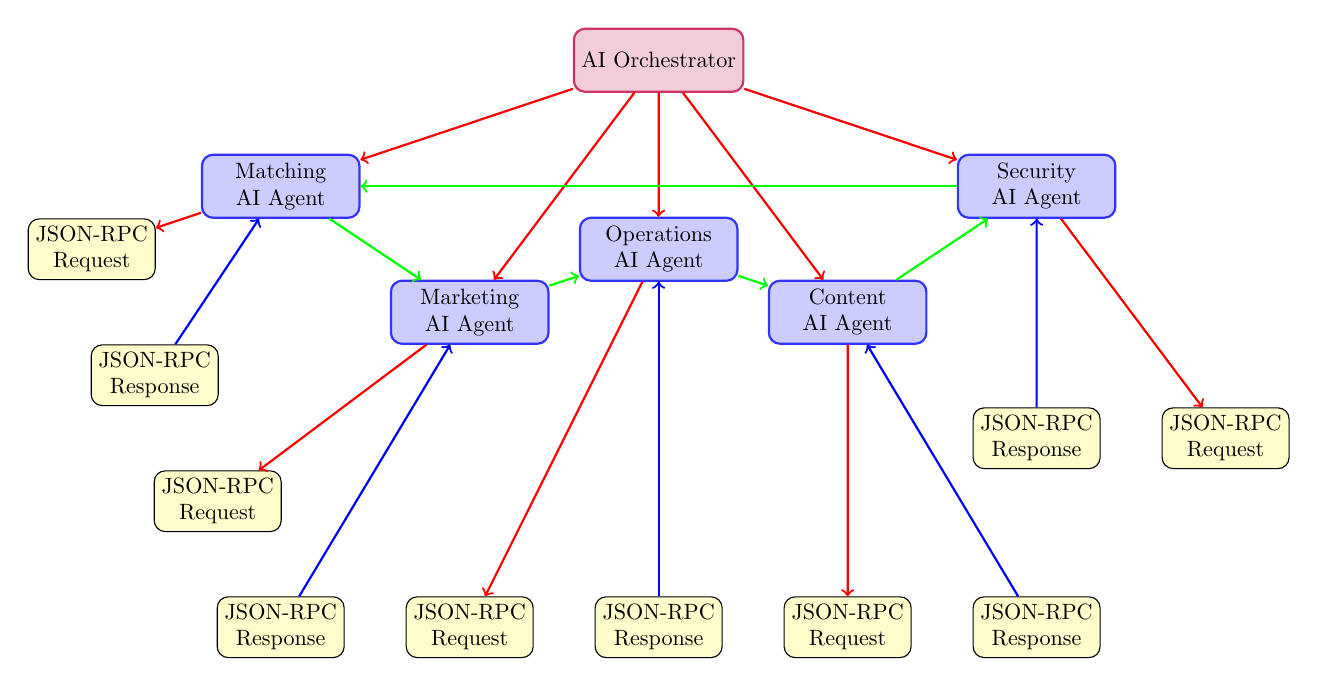
\begin{tikzpicture}[
    scale=0.8,
    transform shape,
    agent/.style={rectangle, draw, rounded corners, minimum width=2.5cm, minimum height=1cm, align=center},
    primary/.style={agent, fill=blue!20, draw=blue!80, thick},
    coordinator/.style={agent, fill=purple!20, draw=purple!80, thick},
    message/.style={rectangle, draw, rounded corners, minimum width=1.5cm, minimum height=0.8cm, align=center, fill=yellow!20},
    arrow/.style={->, thick},
    request/.style={->, thick, red},
    response/.style={->, thick, blue}
]

% AI Agents
\node[coordinator] (orchestrator) at (0,4) {AI Orchestrator};

\node[primary] (matching) at (-6,2) {Matching\\AI Agent};
\node[primary] (marketing) at (-3,0) {Marketing\\AI Agent};
\node[primary] (operations) at (0,1) {Operations\\AI Agent};
\node[primary] (content) at (3,0) {Content\\AI Agent};
\node[primary] (security) at (6,2) {Security\\AI Agent};

% Messages
\node[message] (request1) at (-9,1) {JSON-RPC\\Request};
\node[message] (response1) at (-8,-1) {JSON-RPC\\Response};
\node[message] (request2) at (-7,-3) {JSON-RPC\\Request};
\node[message] (response2) at (-6,-5) {JSON-RPC\\Response};
\node[message] (request3) at (-3,-5) {JSON-RPC\\Request};
\node[message] (response3) at (0,-5) {JSON-RPC\\Response};
\node[message] (request4) at (3,-5) {JSON-RPC\\Request};
\node[message] (response4) at (6,-5) {JSON-RPC\\Response};
\node[message] (request5) at (9,-2) {JSON-RPC\\Request};
\node[message] (response5) at (6,-2) {JSON-RPC\\Response};

% Communication Flow
\draw[request] (orchestrator) -- (matching);
\draw[request] (orchestrator) -- (marketing);
\draw[request] (orchestrator) -- (operations);
\draw[request] (orchestrator) -- (content);
\draw[request] (orchestrator) -- (security);

\draw[request] (matching) -- (request1);
\draw[response] (response1) -- (matching);
\draw[request] (marketing) -- (request2);
\draw[response] (response2) -- (marketing);
\draw[request] (operations) -- (request3);
\draw[response] (response3) -- (operations);
\draw[request] (content) -- (request4);
\draw[response] (response4) -- (content);
\draw[request] (security) -- (request5);
\draw[response] (response5) -- (security);

% Cross-agent communication
\draw[arrow, green] (matching) -- (marketing);
\draw[arrow, green] (marketing) -- (operations);
\draw[arrow, green] (operations) -- (content);
\draw[arrow, green] (content) -- (security);
\draw[arrow, green] (security) -- (matching);

\end{tikzpicture}
\caption{AI Agent Communication Protocol}
\label{fig:ai-communication-protocol}
\end{figure}

\subsection{JSON-RPC Message Format}

The AI agents communicate using a standardized JSON-RPC 2.0 protocol:

\begin{verbatim}
// Request Format
{
  "jsonrpc": "2.0",
  "id": "unique-request-id",
  "method": "agent_method_name",
  "params": {
    "user_id": "user123",
    "context": "matching_request",
    "data": {
      "preferences": {...},
      "constraints": {...}
    }
  }
}

// Response Format
{
  "jsonrpc": "2.0",
  "id": "unique-request-id",
  "result": {
    "success": true,
    "data": {...},
    "confidence": 0.95,
    "metadata": {...}
  },
  "error": null
}
\end{verbatim}

\section{AI Integration and Machine Learning}

\subsection{AI-Powered Platform Features}

The platform integrates advanced AI capabilities to enhance user experience and platform intelligence, building on research from \citep{ferede_artificial_intelligence_ai}.

\subsubsection{Machine Learning Models}

\begin{itemize}
    \item \textbf{Recommendation Systems}: AI-powered member and deal matching algorithms
    \item \textbf{Predictive Analytics}: Forecasting of member behavior and platform trends
    \item \textbf{Natural Language Processing}: Intelligent content analysis and generation
    \item \textbf{Computer Vision}: Image recognition for profile photos and documents
    \item \textbf{Anomaly Detection}: Identification of unusual patterns and potential issues
\end{itemize}

\subsubsection{AI-Powered Automation}

\begin{itemize}
    \item \textbf{Intelligent Member Verification}: AI-enhanced verification processes
    \item \textbf{Automated Content Moderation}: AI-powered content filtering and moderation
    \item \textbf{Smart Notifications}: AI-optimized notification timing and content
    \item \textbf{Predictive Maintenance}: Proactive system monitoring and issue prevention
    \item \textbf{Intelligent Customer Support}: AI-powered support and issue resolution
\end{itemize}

\section{Database Design and Data Architecture}

\subsection{Database Schema Design}

The platform implements a comprehensive database schema optimized for AI operations and real-time processing.

\begin{figure}[h]
\centering
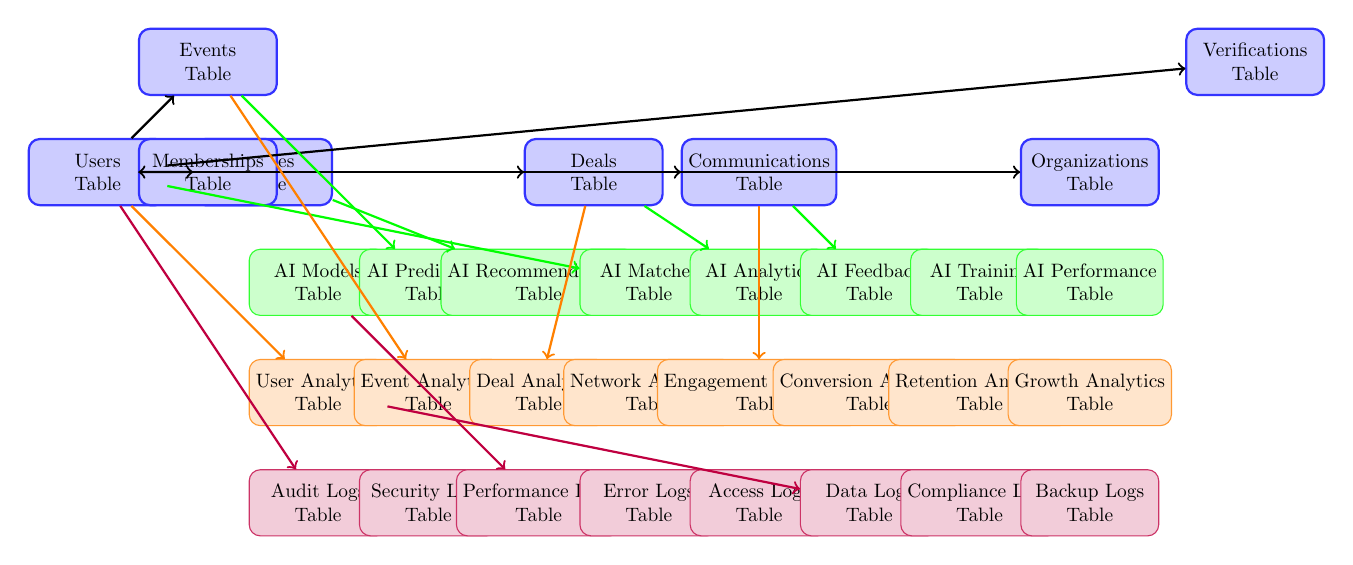
\begin{tikzpicture}[
    scale=0.7,
    transform shape,
    table/.style={rectangle, draw, rounded corners, minimum width=2.5cm, minimum height=1.2cm, align=center},
    core/.style={table, fill=blue!20, draw=blue!80, thick},
    ai/.style={table, fill=green!20, draw=green!80},
    analytics/.style={table, fill=orange!20, draw=orange!80},
    audit/.style={table, fill=purple!20, draw=purple!80},
    arrow/.style={->, thick}
]

% Core Tables
\node[core] (users) at (-12,6) {Users\\Table};
\node[core] (profiles) at (-9,6) {Profiles\\Table};
\node[core] (events) at (-10,8) {Events\\Table};
\node[core] (deals) at (-3,6) {Deals\\Table};
\node[core] (communications) at (0,6) {Communications\\Table};
\node[core] (memberships) at (-10,6) {Memberships\\Table};
\node[core] (organizations) at (6,6) {Organizations\\Table};
\node[core] (verifications) at (9,8) {Verifications\\Table};

% AI Tables
\node[ai] (ai_models) at (-8,4) {AI Models\\Table};
\node[ai] (ai_predictions) at (-6,4) {AI Predictions\\Table};
\node[ai] (ai_recommendations) at (-4,4) {AI Recommendations\\Table};
\node[ai] (ai_matches) at (-2,4) {AI Matches\\Table};
\node[ai] (ai_analytics) at (0,4) {AI Analytics\\Table};
\node[ai] (ai_feedback) at (2,4) {AI Feedback\\Table};
\node[ai] (ai_training) at (4,4) {AI Training\\Table};
\node[ai] (ai_performance) at (6,4) {AI Performance\\Table};

% Analytics Tables
\node[analytics] (user_analytics) at (-8,2) {User Analytics\\Table};
\node[analytics] (event_analytics) at (-6,2) {Event Analytics\\Table};
\node[analytics] (deal_analytics) at (-4,2) {Deal Analytics\\Table};
\node[analytics] (network_analytics) at (-2,2) {Network Analytics\\Table};
\node[analytics] (engagement_analytics) at (0,2) {Engagement Analytics\\Table};
\node[analytics] (conversion_analytics) at (2,2) {Conversion Analytics\\Table};
\node[analytics] (retention_analytics) at (4,2) {Retention Analytics\\Table};
\node[analytics] (growth_analytics) at (6,2) {Growth Analytics\\Table};

% Audit Tables
\node[audit] (audit_logs) at (-8,0) {Audit Logs\\Table};
\node[audit] (security_logs) at (-6,0) {Security Logs\\Table};
\node[audit] (performance_logs) at (-4,0) {Performance Logs\\Table};
\node[audit] (error_logs) at (-2,0) {Error Logs\\Table};
\node[audit] (access_logs) at (0,0) {Access Logs\\Table};
\node[audit] (data_logs) at (2,0) {Data Logs\\Table};
\node[audit] (compliance_logs) at (4,0) {Compliance Logs\\Table};
\node[audit] (backup_logs) at (6,0) {Backup Logs\\Table};

% Relationships
\draw[arrow] (users) -- (profiles);
\draw[arrow] (users) -- (memberships);
\draw[arrow] (users) -- (organizations);
\draw[arrow] (users) -- (verifications);
\draw[arrow] (users) -- (communications);
\draw[arrow] (users) -- (events);
\draw[arrow] (users) -- (deals);

% AI Relationships
\draw[arrow, green] (users) -- (ai_matches);
\draw[arrow, green] (profiles) -- (ai_recommendations);
\draw[arrow, green] (events) -- (ai_predictions);
\draw[arrow, green] (deals) -- (ai_analytics);
\draw[arrow, green] (communications) -- (ai_feedback);

% Analytics Relationships
\draw[arrow, orange] (users) -- (user_analytics);
\draw[arrow, orange] (events) -- (event_analytics);
\draw[arrow, orange] (deals) -- (deal_analytics);
\draw[arrow, orange] (communications) -- (engagement_analytics);

% Audit Relationships
\draw[arrow, purple] (users) -- (audit_logs);
\draw[arrow, purple] (ai_models) -- (performance_logs);
\draw[arrow, purple] (user_analytics) -- (data_logs);

\end{tikzpicture}
\caption{BCD.NET Database Schema Design}
\label{fig:database-schema}
\end{figure}

\subsection{Core Database Tables}

\begin{table}[h]
\centering
\begin{tabular}{|l|l|l|}
\hline
\textbf{Table} & \textbf{Primary Purpose} & \textbf{Key Fields} \\
\hline
users & User authentication and profiles & id, email, password\_hash, status \\
profiles & Detailed user information & user\_id, bio, skills, interests \\
events & Event management & id, title, description, date, location \\
deals & Deal flow management & id, title, description, value, status \\
communications & Messaging system & id, sender\_id, receiver\_id, content \\
memberships & User membership levels & user\_id, level, start\_date, end\_date \\
organizations & Company information & id, name, industry, size \\
verifications & User verification status & user\_id, status, documents \\
\hline
\end{tabular}
\caption{Core Database Tables}
\label{tab:core-database-tables}
\end{table}

\subsection{AI-Specific Database Tables}

\begin{table}[h]
\centering
\begin{tabular}{|l|l|l|}
\hline
\textbf{Table} & \textbf{Purpose} & \textbf{Key Fields} \\
\hline
ai\_models & Model metadata and versions & id, name, version, performance\_metrics \\
ai\_predictions & Prediction results & id, user\_id, prediction\_type, confidence \\
ai\_recommendations & Recommendation data & id, user\_id, item\_id, score, reason \\
ai\_matches & Matching results & id, user1\_id, user2\_id, compatibility\_score \\
ai\_analytics & AI-generated insights & id, data\_source, insight\_type, value \\
ai\_feedback & User feedback on AI & id, user\_id, ai\_action, rating, comment \\
ai\_training & Training data and results & id, model\_id, training\_data, accuracy \\
ai\_performance & Model performance metrics & id, model\_id, metric\_type, value, timestamp \\
\hline
\end{tabular}
\caption{AI-Specific Database Tables}
\label{tab:ai-database-tables}
\end{table}

\section{Data Engineering and Pipeline Architecture}

\subsection{Data Pipeline Architecture}

The platform implements a sophisticated data engineering pipeline for real-time processing and AI model training.

\begin{figure}[h]
\centering
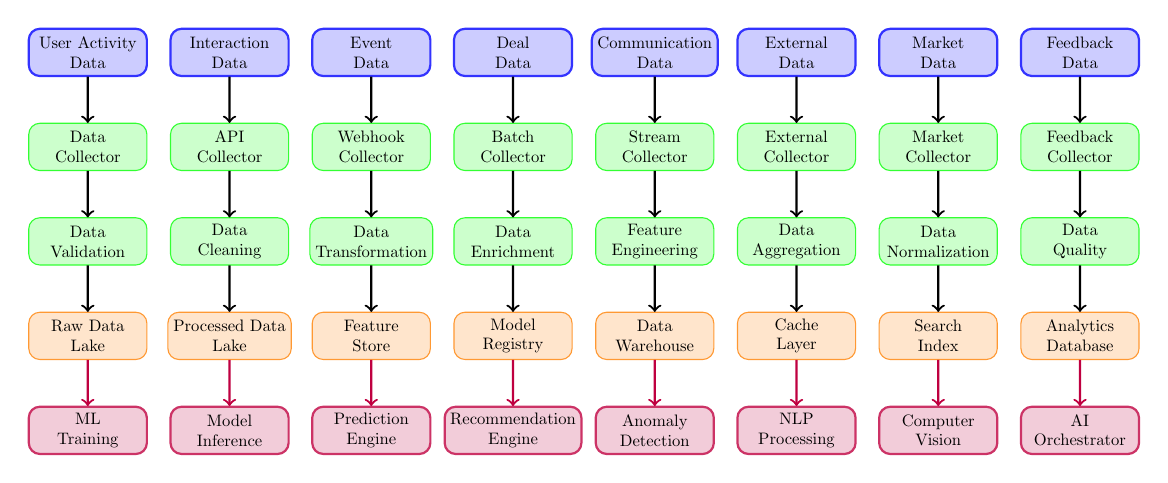
\begin{tikzpicture}[
    scale=0.6,
    transform shape,
    component/.style={rectangle, draw, rounded corners, minimum width=2.5cm, minimum height=1cm, align=center},
    source/.style={component, fill=blue!20, draw=blue!80, thick},
    process/.style={component, fill=green!20, draw=green!80},
    storage/.style={component, fill=orange!20, draw=orange!80},
    ai/.style={component, fill=purple!20, draw=purple!80, thick},
    arrow/.style={->, thick}
]

% Data Sources
\node[source] (user_activity) at (-12,8) {User Activity\\Data};
\node[source] (interaction_data) at (-9,8) {Interaction\\Data};
\node[source] (event_data) at (-6,8) {Event\\Data};
\node[source] (deal_data) at (-3,8) {Deal\\Data};
\node[source] (communication_data) at (0,8) {Communication\\Data};
\node[source] (external_data) at (3,8) {External\\Data};
\node[source] (market_data) at (6,8) {Market\\Data};
\node[source] (feedback_data) at (9,8) {Feedback\\Data};

% Data Collection Layer
\node[process] (data_collector) at (-12,6) {Data\\Collector};
\node[process] (api_collector) at (-9,6) {API\\Collector};
\node[process] (webhook_collector) at (-6,6) {Webhook\\Collector};
\node[process] (batch_collector) at (-3,6) {Batch\\Collector};
\node[process] (stream_collector) at (0,6) {Stream\\Collector};
\node[process] (external_collector) at (3,6) {External\\Collector};
\node[process] (market_collector) at (6,6) {Market\\Collector};
\node[process] (feedback_collector) at (9,6) {Feedback\\Collector};

% Data Processing Layer
\node[process] (data_validation) at (-12,4) {Data\\Validation};
\node[process] (data_cleaning) at (-9,4) {Data\\Cleaning};
\node[process] (data_transformation) at (-6,4) {Data\\Transformation};
\node[process] (data_enrichment) at (-3,4) {Data\\Enrichment};
\node[process] (feature_engineering) at (0,4) {Feature\\Engineering};
\node[process] (data_aggregation) at (3,4) {Data\\Aggregation};
\node[process] (data_normalization) at (6,4) {Data\\Normalization};
\node[process] (data_quality) at (9,4) {Data\\Quality};

% Storage Layer
\node[storage] (raw_data_lake) at (-12,2) {Raw Data\\Lake};
\node[storage] (processed_data_lake) at (-9,2) {Processed Data\\Lake};
\node[storage] (feature_store) at (-6,2) {Feature\\Store};
\node[storage] (model_registry) at (-3,2) {Model\\Registry};
\node[storage] (data_warehouse) at (0,2) {Data\\Warehouse};
\node[storage] (cache_layer) at (3,2) {Cache\\Layer};
\node[storage] (search_index) at (6,2) {Search\\Index};
\node[storage] (analytics_db) at (9,2) {Analytics\\Database};

% AI Processing Layer
\node[ai] (ml_training) at (-12,0) {ML\\Training};
\node[ai] (model_inference) at (-9,0) {Model\\Inference};
\node[ai] (prediction_engine) at (-6,0) {Prediction\\Engine};
\node[ai] (recommendation_engine) at (-3,0) {Recommendation\\Engine};
\node[ai] (anomaly_detection) at (0,0) {Anomaly\\Detection};
\node[ai] (nlp_processing) at (3,0) {NLP\\Processing};
\node[ai] (computer_vision) at (6,0) {Computer\\Vision};
\node[ai] (ai_orchestrator) at (9,0) {AI\\Orchestrator};

% Data Flow
\draw[arrow] (user_activity) -- (data_collector);
\draw[arrow] (interaction_data) -- (api_collector);
\draw[arrow] (event_data) -- (webhook_collector);
\draw[arrow] (deal_data) -- (batch_collector);
\draw[arrow] (communication_data) -- (stream_collector);
\draw[arrow] (external_data) -- (external_collector);
\draw[arrow] (market_data) -- (market_collector);
\draw[arrow] (feedback_data) -- (feedback_collector);

% Processing Flow
\draw[arrow] (data_collector) -- (data_validation);
\draw[arrow] (api_collector) -- (data_cleaning);
\draw[arrow] (webhook_collector) -- (data_transformation);
\draw[arrow] (batch_collector) -- (data_enrichment);
\draw[arrow] (stream_collector) -- (feature_engineering);
\draw[arrow] (external_collector) -- (data_aggregation);
\draw[arrow] (market_collector) -- (data_normalization);
\draw[arrow] (feedback_collector) -- (data_quality);

% Storage Flow
\draw[arrow] (data_validation) -- (raw_data_lake);
\draw[arrow] (data_cleaning) -- (processed_data_lake);
\draw[arrow] (data_transformation) -- (feature_store);
\draw[arrow] (data_enrichment) -- (model_registry);
\draw[arrow] (feature_engineering) -- (data_warehouse);
\draw[arrow] (data_aggregation) -- (cache_layer);
\draw[arrow] (data_normalization) -- (search_index);
\draw[arrow] (data_quality) -- (analytics_db);

% AI Processing Flow
\draw[arrow, purple] (raw_data_lake) -- (ml_training);
\draw[arrow, purple] (processed_data_lake) -- (model_inference);
\draw[arrow, purple] (feature_store) -- (prediction_engine);
\draw[arrow, purple] (model_registry) -- (recommendation_engine);
\draw[arrow, purple] (data_warehouse) -- (anomaly_detection);
\draw[arrow, purple] (cache_layer) -- (nlp_processing);
\draw[arrow, purple] (search_index) -- (computer_vision);
\draw[arrow, purple] (analytics_db) -- (ai_orchestrator);

\end{tikzpicture}
\caption{Data Engineering Pipeline Architecture}
\label{fig:data-pipeline-architecture}
\end{figure}

\subsection{Real-Time Data Processing Specifications}

The platform implements Apache Kafka for real-time data streaming with the following specifications:

\begin{table}[h]
\centering
\begin{tabular}{|l|l|l|}
\hline
\textbf{Kafka Topic} & \textbf{Data Type} & \textbf{Processing Rate} \\
\hline
user-activity & User interactions & 10,000 events/sec \\
user-matches & Matching events & 1,000 events/sec \\
deal-updates & Deal modifications & 500 events/sec \\
event-registrations & Event signups & 2,000 events/sec \\
communication-messages & Chat messages & 5,000 events/sec \\
ai-predictions & AI model outputs & 2,000 predictions/sec \\
ai-feedback & User feedback & 500 feedback/sec \\
system-metrics & Performance metrics & 1,000 metrics/sec \\
\hline
\end{tabular}
\caption{Kafka Topics and Processing Specifications}
\label{tab:kafka-topics}
\end{table}

\subsection{Data Engineering Technologies}

\begin{itemize}
    \item \textbf{Apache Kafka}: Real-time data streaming and event processing
    \item \textbf{Apache Spark}: Large-scale data processing and analytics
    \item \textbf{Apache Airflow}: Workflow orchestration and scheduling
    \item \textbf{Elasticsearch}: Search and analytics engine
    \item \textbf{Redis}: In-memory caching and session storage
    \item \textbf{PostgreSQL}: Primary relational database
    \item \textbf{MongoDB}: Document storage for flexible schemas
    \item \textbf{Apache Cassandra}: Time-series data storage
    \item \textbf{Amazon S3}: Object storage for large datasets
    \item \textbf{MLflow}: Machine learning lifecycle management
\end{itemize}

\section{Security and Compliance}

\subsection{Security Framework}

The platform implements comprehensive security measures, as outlined in \citep{ferede_artificial_intelligence_ai}:

\begin{itemize}
    \item \textbf{Data Encryption}: End-to-end encryption for all sensitive data
    \item \textbf{Access Control}: Role-based access control and authentication
    \item \textbf{Privacy Protection}: GDPR and data protection compliance
    \item \textbf{Security Monitoring}: Continuous security monitoring and threat detection
    \item \textbf{Incident Response}: Rapid response procedures for security incidents
\end{itemize}

\subsection{Compliance and Governance}

\begin{itemize}
    \item \textbf{Data Protection}: Full compliance with GDPR and regional data protection laws
    \item \textbf{Financial Regulations}: Compliance with financial services regulations
    \item \textbf{Audit Trails}: Comprehensive logging for regulatory compliance
    \item \textbf{Privacy Controls}: Granular privacy controls for member data
    \item \textbf{Transparency}: Clear data usage policies and member consent
\end{itemize}

\section{Performance and Scalability}

\subsection{Performance Optimization}

The platform is designed for high performance and scalability, as documented in \:

\begin{itemize}
    \item \textbf{Load Balancing}: Intelligent load distribution across servers
    \item \textbf{Caching Strategy}: Multi-layer caching for optimal performance
    \item \textbf{Database Optimization}: Optimized queries and indexing
    \item \textbf{CDN Integration}: Global content delivery for fast access
    \item \textbf{Real-Time Processing}: Optimized real-time communication
\end{itemize}

\subsection{Scalability Architecture}

\begin{itemize}
    \item \textbf{Microservices Design}: Modular architecture for independent scaling
    \item \textbf{Cloud-Native}: Containerized deployment for easy scaling
    \item \textbf{Auto-Scaling}: Automatic resource allocation based on demand
    \item \textbf{Geographic Distribution}: Multi-region deployment for global access
    \item \textbf{Performance Monitoring}: Real-time performance tracking and optimization
\end{itemize}

\section{AI Agent-Based Pairing Mechanism}

\subsection{Intelligent Matching Algorithm}
The AI-powered pairing system represents a breakthrough in networking efficiency, designed to facilitate meaningful connections based on multiple criteria beyond simple industry matching.

\subsubsection{Matching Criteria}
\begin{itemize}
    \item \textbf{Business Profile}: Company size, industry, growth stage
    \item \textbf{Investment Interests}: Deal flow preferences, investment thesis
    \item \textbf{Geographic Focus}: Regional expertise and market knowledge
    \item \textbf{Professional Background}: Experience level, expertise areas
    \item \textbf{Networking Goals}: Specific objectives and desired outcomes
    \item \textbf{Compatibility Factors}: Communication style, meeting preferences
\end{itemize}

\subsubsection{AI Algorithm Components}
\begin{itemize}
    \item \textbf{Machine Learning Models}: Supervised learning for connection success prediction
    \item \textbf{Natural Language Processing}: Analysis of member profiles and preferences
    \item \textbf{Recommendation Engine}: Collaborative filtering and content-based filtering
    \item \textbf{Real-time Learning}: Continuous improvement based on user feedback
    \item \textbf{Privacy-Preserving Matching}: Secure data handling and anonymization
\end{itemize}

\subsection{Shadow Learning from Top Performers}
The most effective AI agent development strategy involves shadowing top performers and codifying their decision-making processes into concrete, actionable frameworks.

\begin{figure}[h]
\centering
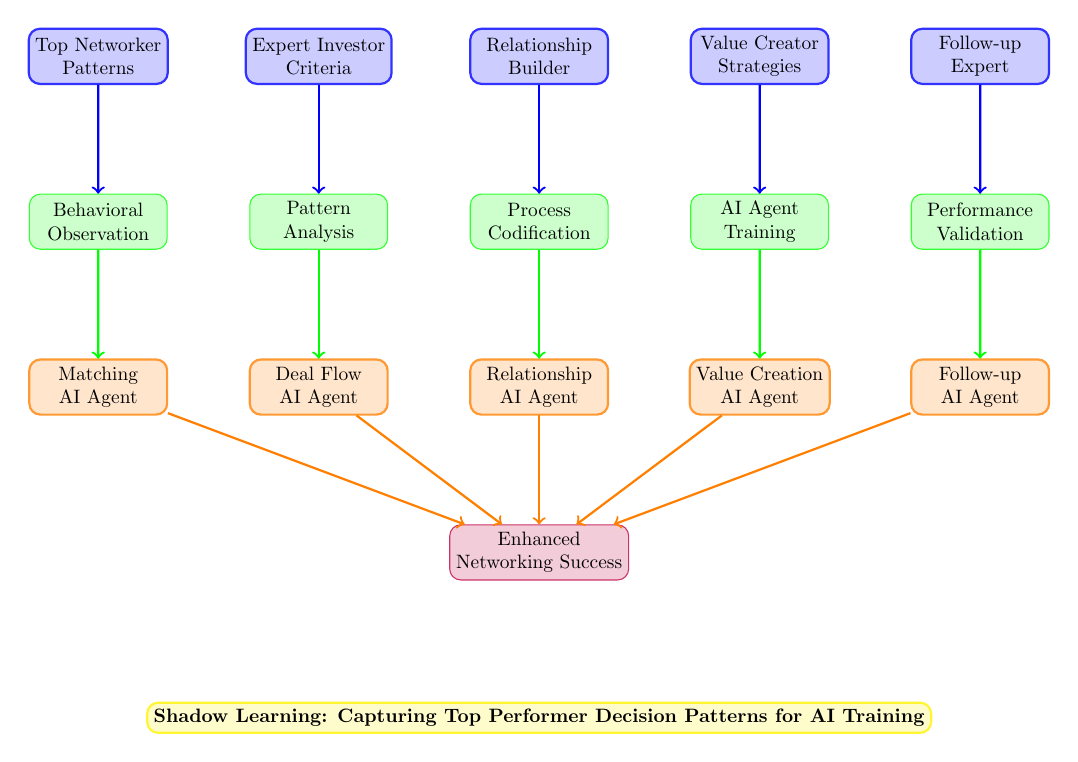
\begin{tikzpicture}[
    scale=0.7,
    transform shape,
    box/.style={rectangle, draw, rounded corners, minimum width=2.5cm, minimum height=1cm, align=center},
    performer/.style={box, fill=blue!20, draw=blue!80, thick},
    process/.style={box, fill=green!20, draw=green!80},
    ai/.style={box, fill=orange!20, draw=orange!80, thick},
    outcome/.style={box, fill=purple!20, draw=purple!80},
    arrow/.style={->, thick}
]

% Top Performers
\node[performer] (networker) at (-8,4) {Top Networker\\Patterns};
\node[performer] (investor) at (-4,4) {Expert Investor\\Criteria};
\node[performer] (relationship) at (0,4) {Relationship\\Builder};
\node[performer] (value) at (4,4) {Value Creator\\Strategies};
\node[performer] (followup) at (8,4) {Follow-up\\Expert};

% Learning Process
\node[process] (observation) at (-8,1) {Behavioral\\Observation};
\node[process] (analysis) at (-4,1) {Pattern\\Analysis};
\node[process] (codification) at (0,1) {Process\\Codification};
\node[process] (training) at (4,1) {AI Agent\\Training};
\node[process] (validation) at (8,1) {Performance\\Validation};

% AI Agents
\node[ai] (matching_ai) at (-8,-2) {Matching\\AI Agent};
\node[ai] (deal_ai) at (-4,-2) {Deal Flow\\AI Agent};
\node[ai] (relationship_ai) at (0,-2) {Relationship\\AI Agent};
\node[ai] (value_ai) at (4,-2) {Value Creation\\AI Agent};
\node[ai] (followup_ai) at (8,-2) {Follow-up\\AI Agent};

% Outcomes
\node[outcome] (success) at (0,-5) {Enhanced\\Networking Success};

% Learning flow
\draw[arrow, blue] (networker) -- (observation);
\draw[arrow, blue] (investor) -- (analysis);
\draw[arrow, blue] (relationship) -- (codification);
\draw[arrow, blue] (value) -- (training);
\draw[arrow, blue] (followup) -- (validation);

% Process flow
\draw[arrow, green] (observation) -- (matching_ai);
\draw[arrow, green] (analysis) -- (deal_ai);
\draw[arrow, green] (codification) -- (relationship_ai);
\draw[arrow, green] (training) -- (value_ai);
\draw[arrow, green] (validation) -- (followup_ai);

% AI outcomes
\draw[arrow, orange] (matching_ai) -- (success);
\draw[arrow, orange] (deal_ai) -- (success);
\draw[arrow, orange] (relationship_ai) -- (success);
\draw[arrow, orange] (value_ai) -- (success);
\draw[arrow, orange] (followup_ai) -- (success);

% Shadow learning highlight
\node[fill=yellow!20, draw=yellow!80, thick, rounded corners] at (0,-8) 
    {\textbf{Shadow Learning: Capturing Top Performer Decision Patterns for AI Training}};

\end{tikzpicture}
\caption{AI Agent Shadow Learning Process from Top Performers}
\label{fig:shadow-learning-process}
\end{figure}

\subsubsection{Top Performer Analysis}
\begin{itemize}
    \item \textbf{Network Building Patterns}: How successful members identify and approach potential connections
    \item \textbf{Deal Flow Assessment}: Criteria used by experienced investors to evaluate opportunities
    \item \textbf{Relationship Development}: Strategies for building and maintaining professional relationships
    \item \textbf{Value Creation}: Methods for creating mutual value in networking interactions
    \item \textbf{Follow-up Strategies}: Systematic approaches to maintaining connection momentum
\end{itemize}

\subsubsection{AI Agent Training Framework}
\begin{itemize}
    \item \textbf{Behavioral Modeling}: Capturing decision patterns from successful networkers
    \item \textbf{Scenario Training}: Teaching AI agents to handle various networking situations
    \item \textbf{Feedback Integration}: Continuous learning from member interactions and outcomes
    \item \textbf{Ethical Guidelines}: Ensuring AI recommendations align with BCD's values
    \item \textbf{Performance Metrics}: Measuring AI agent effectiveness in facilitating successful connections
\end{itemize}

\section{AI-Powered Business Operations}

\subsection{Marketing Strategy AI Agent}
The development of AI agents for marketing strategy represents a significant opportunity to enhance BCD's competitive positioning and growth initiatives.

\subsubsection{Market Intelligence Analysis}
\begin{itemize}
    \item \textbf{Competitive Monitoring}: Automated tracking of competitor activities and positioning
    \item \textbf{Market Trend Analysis}: Real-time identification of emerging opportunities and threats
    \item \textbf{Member Sentiment Analysis}: Understanding member needs and satisfaction levels
    \item \textbf{Content Performance Optimization}: AI-driven content strategy and optimization
    \item \textbf{Lead Generation Intelligence}: Identifying high-potential prospects and engagement opportunities
\end{itemize}

\subsubsection{Personalized Marketing Automation}
\begin{itemize}
    \item \textbf{Member Segmentation}: AI-powered member categorization and targeting
    \item \textbf{Content Personalization}: Tailored messaging and content delivery
    \item \textbf{Engagement Optimization}: Automated follow-up and relationship nurturing
    \item \textbf{Event Recommendation}: Intelligent suggestions for member participation
    \item \textbf{Referral Optimization}: AI-enhanced member referral program management
\end{itemize}

\subsection{Business Operations AI Agent}
AI agents can significantly enhance BCD's operational efficiency and decision-making processes.

\subsubsection{Operational Intelligence}
\begin{itemize}
    \item \textbf{Performance Analytics}: Real-time monitoring of key business metrics
    \item \textbf{Predictive Modeling}: Forecasting member growth, retention, and revenue trends
    \item \textbf{Resource Optimization}: AI-driven allocation of marketing and operational resources
    \item \textbf{Risk Assessment}: Automated identification of potential business risks and opportunities
    \item \textbf{Process Automation}: Streamlining repetitive operational tasks
\end{itemize}

\subsubsection{Strategic Decision Support}
\begin{itemize}
    \item \textbf{Market Entry Analysis}: AI-powered evaluation of expansion opportunities
    \item \textbf{Partnership Assessment}: Automated analysis of potential strategic partnerships
    \item \textbf{Investment Prioritization}: AI-driven resource allocation for platform development
    \item \textbf{Competitive Response Planning}: Automated monitoring and response to competitive threats
    \item \textbf{Scenario Planning}: AI-powered modeling of different business scenarios and outcomes
\end{itemize}

\section{Detailed Implementation Specifications}

\subsection{AI Agent Implementation Architecture}

Each AI agent is implemented as a microservice with specific responsibilities and communication protocols.

\begin{figure}[h]
\centering
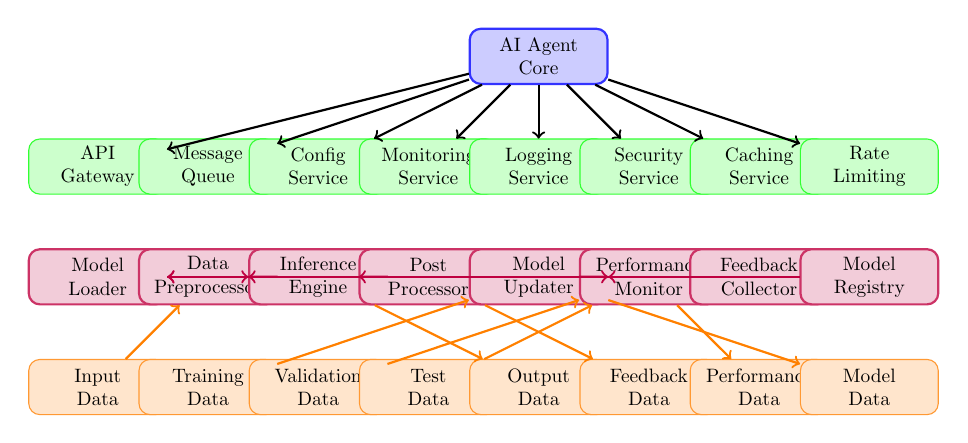
\begin{tikzpicture}[
    scale=0.7,
    transform shape,
    component/.style={rectangle, draw, rounded corners, minimum width=2.5cm, minimum height=1cm, align=center},
    agent/.style={component, fill=blue!20, draw=blue!80, thick},
    service/.style={component, fill=green!20, draw=green!80},
    data/.style={component, fill=orange!20, draw=orange!80},
    ml/.style={component, fill=purple!20, draw=purple!80, thick},
    arrow/.style={->, thick}
]

% AI Agent Core
\node[agent] (agent_core) at (0,6) {AI Agent\\Core};

% Agent Services
\node[service] (api_gateway) at (-8,4) {API\\Gateway};
\node[service] (message_queue) at (-6,4) {Message\\Queue};
\node[service] (config_service) at (-4,4) {Config\\Service};
\node[service] (monitoring) at (-2,4) {Monitoring\\Service};
\node[service] (logging) at (0,4) {Logging\\Service};
\node[service] (security) at (2,4) {Security\\Service};
\node[service] (caching) at (4,4) {Caching\\Service};
\node[service] (rate_limiting) at (6,4) {Rate\\Limiting};

% ML Components
\node[ml] (model_loader) at (-8,2) {Model\\Loader};
\node[ml] (preprocessor) at (-6,2) {Data\\Preprocessor};
\node[ml] (inference_engine) at (-4,2) {Inference\\Engine};
\node[ml] (postprocessor) at (-2,2) {Post\\Processor};
\node[ml] (model_updater) at (0,2) {Model\\Updater};
\node[ml] (performance_monitor) at (2,2) {Performance\\Monitor};
\node[ml] (feedback_collector) at (4,2) {Feedback\\Collector};
\node[ml] (model_registry) at (6,2) {Model\\Registry};

% Data Sources
\node[data] (input_data) at (-8,0) {Input\\Data};
\node[data] (training_data) at (-6,0) {Training\\Data};
\node[data] (validation_data) at (-4,0) {Validation\\Data};
\node[data] (test_data) at (-2,0) {Test\\Data};
\node[data] (output_data) at (0,0) {Output\\Data};
\node[data] (feedback_data) at (2,0) {Feedback\\Data};
\node[data] (performance_data) at (4,0) {Performance\\Data};
\node[data] (model_data) at (6,0) {Model\\Data};

% Connections
\draw[arrow] (agent_core) -- (api_gateway);
\draw[arrow] (agent_core) -- (message_queue);
\draw[arrow] (agent_core) -- (config_service);
\draw[arrow] (agent_core) -- (monitoring);
\draw[arrow] (agent_core) -- (logging);
\draw[arrow] (agent_core) -- (security);
\draw[arrow] (agent_core) -- (caching);
\draw[arrow] (agent_core) -- (rate_limiting);

% ML connections
\draw[arrow, purple] (model_loader) -- (inference_engine);
\draw[arrow, purple] (preprocessor) -- (inference_engine);
\draw[arrow, purple] (inference_engine) -- (postprocessor);
\draw[arrow, purple] (model_updater) -- (model_loader);
\draw[arrow, purple] (performance_monitor) -- (model_updater);
\draw[arrow, purple] (feedback_collector) -- (model_updater);
\draw[arrow, purple] (model_registry) -- (model_loader);

% Data connections
\draw[arrow, orange] (input_data) -- (preprocessor);
\draw[arrow, orange] (training_data) -- (model_updater);
\draw[arrow, orange] (validation_data) -- (performance_monitor);
\draw[arrow, orange] (test_data) -- (performance_monitor);
\draw[arrow, orange] (inference_engine) -- (output_data);
\draw[arrow, orange] (postprocessor) -- (feedback_data);
\draw[arrow, orange] (performance_monitor) -- (performance_data);
\draw[arrow, orange] (model_updater) -- (model_data);

\end{tikzpicture}
\caption{AI Agent Implementation Architecture}
\label{fig:ai-agent-implementation}
\end{figure}

\subsection{Code Implementation Examples}

\subsubsection{AI Agent Base Class (Python)}

\begin{verbatim}
import asyncio
import json
import logging
from typing import Dict, Any, Optional
from abc import ABC, abstractmethod
import aiohttp
import redis
from prometheus_client import Counter, Histogram

class BaseAIAgent(ABC):
    """Base class for all AI agents in the BCD.NET platform."""
    
    def __init__(self, agent_name: str, config: Dict[str, Any]):
        self.agent_name = agent_name
        self.config = config
        self.logger = logging.getLogger(f"ai_agent.{agent_name}")
        self.redis_client = redis.Redis(
            host=config['redis_host'],
            port=config['redis_port'],
            db=config['redis_db']
        )
        
        # Prometheus metrics
        self.request_counter = Counter(
            f'{agent_name}_requests_total',
            'Total requests processed'
        )
        self.processing_time = Histogram(
            f'{agent_name}_processing_seconds',
            'Request processing time'
        )
        
    @abstractmethod
    async def process_request(self, request_data: Dict[str, Any]) -> Dict[str, Any]:
        """Process incoming request and return response."""
        pass
    
    @abstractmethod
    async def load_model(self) -> bool:
        """Load the AI model for this agent."""
        pass
    
    async def handle_request(self, request: Dict[str, Any]) -> Dict[str, Any]:
        """Handle incoming JSON-RPC request."""
        try:
            self.request_counter.inc()
            
            with self.processing_time.time():
                result = await self.process_request(request['params'])
            
            return {
                "jsonrpc": "2.0",
                "id": request.get('id'),
                "result": {
                    "success": True,
                    "data": result,
                    "confidence": result.get('confidence', 0.0),
                    "metadata": {
                        "agent": self.agent_name,
                        "timestamp": asyncio.get_event_loop().time()
                    }
                },
                "error": None
            }
        except Exception as e:
            self.logger.error(f"Error processing request: {e}")
            return {
                "jsonrpc": "2.0",
                "id": request.get('id'),
                "result": None,
                "error": {
                    "code": -32603,
                    "message": str(e)
                }
            }
    
    async def cache_result(self, key: str, data: Any, ttl: int = 3600):
        """Cache result in Redis."""
        await self.redis_client.setex(
            f"{self.agent_name}:{key}",
            ttl,
            json.dumps(data)
        )
    
    async def get_cached_result(self, key: str) -> Optional[Dict[str, Any]]:
        """Get cached result from Redis."""
        cached = await self.redis_client.get(f"{self.agent_name}:{key}")
        return json.loads(cached) if cached else None
\end{verbatim}

\subsubsection{Matching AI Agent Implementation}

\begin{verbatim}
import numpy as np
import pandas as pd
from sklearn.ensemble import RandomForestClassifier
from sklearn.feature_extraction.text import TfidfVectorizer
from typing import List, Dict, Any
import asyncio

class MatchingAIAgent(BaseAIAgent):
    """AI Agent for member matching and recommendations."""
    
    def __init__(self, config: Dict[str, Any]):
        super().__init__("matching_ai", config)
        self.model = None
        self.vectorizer = TfidfVectorizer(max_features=1000)
        self.feature_columns = [
            'industry', 'company_size', 'experience_level',
            'investment_interests', 'geographic_focus'
        ]
    
    async def load_model(self) -> bool:
        """Load the matching model."""
        try:
            # Load pre-trained model from model registry
            model_path = self.config['model_path']
            self.model = RandomForestClassifier()
            # Load model weights here
            self.logger.info("Matching model loaded successfully")
            return True
        except Exception as e:
            self.logger.error(f"Failed to load model: {e}")
            return False
    
    async def process_request(self, request_data: Dict[str, Any]) -> Dict[str, Any]:
        """Process matching request."""
        user_id = request_data['user_id']
        preferences = request_data.get('preferences', {})
        constraints = request_data.get('constraints', {})
        
        # Check cache first
        cache_key = f"match_{user_id}_{hash(str(preferences))}"
        cached_result = await self.get_cached_result(cache_key)
        if cached_result:
            return cached_result
        
        # Get user profile
        user_profile = await self._get_user_profile(user_id)
        
        # Get potential matches
        potential_matches = await self._get_potential_matches(
            user_profile, preferences, constraints
        )
        
        # Calculate compatibility scores
        compatibility_scores = await self._calculate_compatibility(
            user_profile, potential_matches
        )
        
        # Generate recommendations
        recommendations = await self._generate_recommendations(
            potential_matches, compatibility_scores
        )
        
        result = {
            "user_id": user_id,
            "recommendations": recommendations,
            "confidence": np.mean([r['score'] for r in recommendations]),
            "total_matches": len(recommendations),
            "processing_time": asyncio.get_event_loop().time()
        }
        
        # Cache result
        await self.cache_result(cache_key, result, ttl=1800)
        
        return result
    
    async def _get_user_profile(self, user_id: str) -> Dict[str, Any]:
        """Retrieve user profile from database."""
        # Implementation for database query
        pass
    
    async def _get_potential_matches(
        self, 
        user_profile: Dict[str, Any], 
        preferences: Dict[str, Any], 
        constraints: Dict[str, Any]
    ) -> List[Dict[str, Any]]:
        """Get potential matches based on criteria."""
        # Implementation for filtering potential matches
        pass
    
    async def _calculate_compatibility(
        self, 
        user_profile: Dict[str, Any], 
        potential_matches: List[Dict[str, Any]]
    ) -> List[float]:
        """Calculate compatibility scores using ML model."""
        # Feature engineering
        features = []
        for match in potential_matches:
            feature_vector = self._extract_features(user_profile, match)
            features.append(feature_vector)
        
        # Model prediction
        if self.model:
            scores = self.model.predict_proba(features)[:, 1]
        else:
            # Fallback to simple scoring
            scores = [0.5] * len(potential_matches)
        
        return scores.tolist()
    
    def _extract_features(
        self, 
        user_profile: Dict[str, Any], 
        match_profile: Dict[str, Any]
    ) -> List[float]:
        """Extract features for compatibility prediction."""
        features = []
        
        # Industry compatibility
        industry_match = 1.0 if user_profile['industry'] == match_profile['industry'] else 0.0
        features.append(industry_match)
        
        # Company size compatibility
        size_diff = abs(user_profile['company_size'] - match_profile['company_size'])
        size_compatibility = 1.0 / (1.0 + size_diff)
        features.append(size_compatibility)
        
        # Experience level compatibility
        exp_diff = abs(user_profile['experience_level'] - match_profile['experience_level'])
        exp_compatibility = 1.0 / (1.0 + exp_diff)
        features.append(exp_compatibility)
        
        # Investment interests overlap
        user_interests = set(user_profile.get('investment_interests', []))
        match_interests = set(match_profile.get('investment_interests', []))
        interest_overlap = len(user_interests & match_interests) / max(len(user_interests), 1)
        features.append(interest_overlap)
        
        # Geographic compatibility
        geo_match = 1.0 if user_profile['geographic_focus'] == match_profile['geographic_focus'] else 0.0
        features.append(geo_match)
        
        return features
    
    async def _generate_recommendations(
        self, 
        potential_matches: List[Dict[str, Any]], 
        compatibility_scores: List[float]
    ) -> List[Dict[str, Any]]:
        """Generate final recommendations."""
        recommendations = []
        
        for match, score in zip(potential_matches, compatibility_scores):
            if score > 0.3:  # Minimum compatibility threshold
                recommendation = {
                    "user_id": match['id'],
                    "name": match['name'],
                    "company": match['company'],
                    "score": float(score),
                    "reason": self._generate_reason(match, score),
                    "contact_info": match.get('contact_info', {})
                }
                recommendations.append(recommendation)
        
        # Sort by score and limit to top 10
        recommendations.sort(key=lambda x: x['score'], reverse=True)
        return recommendations[:10]
    
    def _generate_reason(self, match: Dict[str, Any], score: float) -> str:
        """Generate explanation for recommendation."""
        reasons = []
        
        if score > 0.8:
            reasons.append("High compatibility based on multiple factors")
        elif score > 0.6:
            reasons.append("Good compatibility with complementary skills")
        else:
            reasons.append("Moderate compatibility with potential synergies")
        
        return "; ".join(reasons)
\end{verbatim}

\subsubsection{API Gateway Configuration (YAML)}

\begin{verbatim}
# kong.yml
_format_version: "2.1"
_transform: true

services:
  - name: matching-ai-service
    url: http://matching-ai-agent:8000
    routes:
      - name: matching-ai-route
        paths:
          - /api/v1/ai/matching
        methods:
          - POST
        plugins:
          - name: rate-limiting
            config:
              minute: 100
              hour: 1000
          - name: key-auth
            config:
              key_names:
                - apikey
              hide_credentials: true
          - name: prometheus
            config:
              status_codes: true
              latency: true
              bandwidth: true
              upstream_health: true

  - name: marketing-ai-service
    url: http://marketing-ai-agent:8000
    routes:
      - name: marketing-ai-route
        paths:
          - /api/v1/ai/marketing
        methods:
          - POST
        plugins:
          - name: rate-limiting
            config:
              minute: 50
              hour: 500
          - name: key-auth
            config:
              key_names:
                - apikey
              hide_credentials: true

  - name: operations-ai-service
    url: http://operations-ai-agent:8000
    routes:
      - name: operations-ai-route
        paths:
          - /api/v1/ai/operations
        methods:
          - POST
        plugins:
          - name: rate-limiting
            config:
              minute: 75
              hour: 750
          - name: key-auth
            config:
              key_names:
                - apikey
              hide_credentials: true

consumers:
  - username: bcd-platform
    keyauth_credentials:
      - key: "bcd-ai-platform-key-2024"
    acl_groups:
      - ai-agents

plugins:
  - name: prometheus
    config:
      status_codes: true
      latency: true
      bandwidth: true
      upstream_health: true
  - name: cors
    config:
      origins:
        - "https://bcd.network"
        - "https://app.bcd.network"
      methods:
        - GET
        - POST
        - PUT
        - DELETE
        - OPTIONS
      headers:
        - Content-Type
        - Authorization
        - X-Requested-With
      exposed_headers:
        - X-Total-Count
      credentials: true
      max_age: 3600
\end{verbatim}

\subsubsection{Docker Compose Configuration}

\begin{verbatim}
# docker-compose.yml
version: '3.8'

services:
  # API Gateway
  api-gateway:
    image: kong:3.4
    ports:
      - "8000:8000"
      - "8443:8443"
    environment:
      KONG_DATABASE: postgres
      KONG_PG_HOST: postgres
      KONG_PG_DATABASE: kong
      KONG_PG_USER: kong
      KONG_PG_PASSWORD: kong_password
    volumes:
      - ./kong.yml:/kong.yml
    depends_on:
      - postgres
    networks:
      - bcd-network

  # AI Agents
  matching-ai-agent:
    build:
      context: ./ai-agents/matching
      dockerfile: Dockerfile
    environment:
      - REDIS_HOST=redis
      - REDIS_PORT=6379
      - MODEL_PATH=/models/matching_model.pkl
      - LOG_LEVEL=INFO
    volumes:
      - ./models:/models
      - ./logs:/logs
    depends_on:
      - redis
      - postgres
    networks:
      - bcd-network
    deploy:
      resources:
        limits:
          memory: 2G
          cpus: '1.0'
        reservations:
          memory: 1G
          cpus: '0.5'

  marketing-ai-agent:
    build:
      context: ./ai-agents/marketing
      dockerfile: Dockerfile
    environment:
      - REDIS_HOST=redis
      - REDIS_PORT=6379
      - MODEL_PATH=/models/marketing_model.pkl
      - LOG_LEVEL=INFO
    volumes:
      - ./models:/models
      - ./logs:/logs
    depends_on:
      - redis
      - postgres
    networks:
      - bcd-network
    deploy:
      resources:
        limits:
          memory: 2G
          cpus: '1.0'
        reservations:
          memory: 1G
          cpus: '0.5'

  operations-ai-agent:
    build:
      context: ./ai-agents/operations
      dockerfile: Dockerfile
    environment:
      - REDIS_HOST=redis
      - REDIS_PORT=6379
      - MODEL_PATH=/models/operations_model.pkl
      - LOG_LEVEL=INFO
    volumes:
      - ./models:/models
      - ./logs:/logs
    depends_on:
      - redis
      - postgres
    networks:
      - bcd-network
    deploy:
      resources:
        limits:
          memory: 2G
          cpus: '1.0'
        reservations:
          memory: 1G
          cpus: '0.5'

  # Data Infrastructure
  postgres:
    image: postgres:15
    environment:
      POSTGRES_DB: bcd_platform
      POSTGRES_USER: bcd_user
      POSTGRES_PASSWORD: bcd_password
    volumes:
      - postgres_data:/var/lib/postgresql/data
      - ./init.sql:/docker-entrypoint-initdb.d/init.sql
    ports:
      - "5432:5432"
    networks:
      - bcd-network

  redis:
    image: redis:7-alpine
    ports:
      - "6379:6379"
    volumes:
      - redis_data:/data
    networks:
      - bcd-network

  elasticsearch:
    image: elasticsearch:8.8.0
    environment:
      - discovery.type=single-node
      - xpack.security.enabled=false
    ports:
      - "9200:9200"
    volumes:
      - elasticsearch_data:/usr/share/elasticsearch/data
    networks:
      - bcd-network

  kafka:
    image: confluentinc/cp-kafka:7.4.0
    ports:
      - "9092:9092"
    environment:
      KAFKA_ZOOKEEPER_CONNECT: zookeeper:2181
      KAFKA_ADVERTISED_LISTENERS: PLAINTEXT://kafka:29092,PLAINTEXT_HOST://localhost:9092
      KAFKA_LISTENER_SECURITY_PROTOCOL_MAP: PLAINTEXT:PLAINTEXT,PLAINTEXT_HOST:PLAINTEXT
      KAFKA_INTER_BROKER_LISTENER_NAME: PLAINTEXT
      KAFKA_OFFSETS_TOPIC_REPLICATION_FACTOR: 1
    depends_on:
      - zookeeper
    networks:
      - bcd-network

  zookeeper:
    image: confluentinc/cp-zookeeper:7.4.0
    environment:
      ZOOKEEPER_CLIENT_PORT: 2181
      ZOOKEEPER_TICK_TIME: 2000
    networks:
      - bcd-network

  # Monitoring
  prometheus:
    image: prom/prometheus:latest
    ports:
      - "9090:9090"
    volumes:
      - ./prometheus.yml:/etc/prometheus/prometheus.yml
      - prometheus_data:/prometheus
    networks:
      - bcd-network

  grafana:
    image: grafana/grafana:latest
    ports:
      - "3000:3000"
    environment:
      - GF_SECURITY_ADMIN_PASSWORD=admin
    volumes:
      - grafana_data:/var/lib/grafana
    networks:
      - bcd-network

volumes:
  postgres_data:
  redis_data:
  elasticsearch_data:
  prometheus_data:
  grafana_data:

networks:
  bcd-network:
    driver: bridge
\end{verbatim}

\section{Implementation Roadmap}

\subsection{Phase 1: Foundation (Months 1-6)}
\begin{itemize}
    \item \textbf{Platform Development}: Core BCD.NET platform with basic member management
    \item \textbf{Data Infrastructure}: Secure data collection and storage systems
    \item \textbf{Basic AI Integration}: Simple recommendation algorithms and matching
    \item \textbf{User Testing}: Member feedback and platform optimization
    \item \textbf{Security Implementation}: Comprehensive data protection and privacy measures
\end{itemize}

\subsection{Phase 2: AI Enhancement (Months 7-18)}
\begin{itemize}
    \item \textbf{Advanced Matching}: Sophisticated AI-powered pairing algorithms
    \item \textbf{Marketing AI}: Automated marketing strategy and content optimization
    \item \textbf{Operational AI}: Business intelligence and decision support systems
    \item \textbf{Mobile Application}: Native mobile app for enhanced user experience
    \item \textbf{API Integration}: Third-party service integrations and partnerships
\end{itemize}

\subsection{Phase 3: Advanced Features (Months 19-36)}
\begin{itemize}
    \item \textbf{Predictive Analytics}: Advanced forecasting and trend analysis
    \item \textbf{Automated Deal Flow}: AI-powered deal discovery and matching
    \item \textbf{Virtual Events Platform}: Comprehensive hybrid event management
    \item \textbf{Advanced Security}: Blockchain-based verification and trust systems
    \item \textbf{Global Expansion}: Multi-language and multi-region platform support
\end{itemize}

\section{Technical Considerations}

\subsection{Scalability and Performance}
\begin{itemize}
    \item \textbf{Microservices Architecture}: Modular design for easy scaling and maintenance
    \item \textbf{Cloud-Native Development}: Containerized deployment for flexibility
    \item \textbf{Database Optimization}: Efficient data storage and retrieval systems
    \item \textbf{CDN Integration}: Global content delivery for optimal performance
    \item \textbf{Load Balancing}: Automated traffic distribution and failover systems
\end{itemize}

\subsection{Security and Privacy}
\begin{itemize}
    \item \textbf{Data Encryption}: End-to-end encryption for sensitive information
    \item \textbf{GDPR Compliance}: Full compliance with European data protection regulations
    \item \textbf{Access Control}: Role-based permissions and authentication
    \item \textbf{Audit Trails}: Comprehensive logging and monitoring systems
    \item \textbf{Regular Security Audits}: Ongoing vulnerability assessment and remediation
\end{itemize}

\subsection{AI Ethics and Governance}
\begin{itemize}
    \item \textbf{Transparency}: Clear explanation of AI decision-making processes
    \item \textbf{Fairness}: Ensuring AI algorithms don't perpetuate biases
    \item \textbf{Accountability}: Human oversight and control of AI systems
    \item \textbf{Privacy Protection}: Minimizing data collection and ensuring user control
    \item \textbf{Continuous Monitoring}: Regular assessment of AI system performance and impact
\end{itemize}

\section{Success Metrics and KPIs}

\subsection{Platform Performance Metrics}
\begin{itemize}
    \item \textbf{User Engagement}: Daily active users, session duration, feature adoption
    \item \textbf{Connection Success Rate}: Percentage of AI-suggested connections that result in meaningful interactions
    \item \textbf{Platform Reliability}: Uptime, response time, error rates
    \item \textbf{Member Satisfaction}: Net Promoter Score and user feedback scores
    \item \textbf{Deal Flow Integration}: Number of deals posted and successfully matched
\end{itemize}

\subsection{AI Effectiveness Metrics}
\begin{itemize}
    \item \textbf{Matching Accuracy}: Success rate of AI-powered connection suggestions
    \item \textbf{Learning Efficiency}: Rate of AI model improvement over time
    \item \textbf{User Adoption}: Percentage of members using AI-powered features
    \item \textbf{Business Impact}: Correlation between AI usage and member success metrics
    \item \textbf{Ethical Compliance}: Monitoring for bias and fairness in AI recommendations
\end{itemize}

\section{Investment Requirements}

\subsection{Development Costs}
\begin{itemize}
    \item \textbf{Platform Development}: €500,000 - €1,000,000 for full-featured platform
    \item \textbf{AI Integration}: €200,000 - €400,000 for advanced AI capabilities
    \item \textbf{Security Implementation}: €100,000 - €200,000 for comprehensive security
    \item \textbf{Testing and Quality Assurance}: €150,000 - €300,000 for thorough testing
    \item \textbf{Deployment and Infrastructure}: €100,000 - €200,000 for cloud infrastructure
\end{itemize}
\subsection{Ongoing Operational Costs}
\begin{itemize}
    \item \textbf{Platform Maintenance}: €50,000 - €100,000 annually
    \item \textbf{AI Model Training}: €30,000 - €60,000 annually
    \item \textbf{Security Monitoring}: €20,000 - €40,000 annually
    \item \textbf{Cloud Infrastructure}: €40,000 - €80,000 annually
    \item \textbf{Technical Support}: €30,000 - €60,000 annually
\end{itemize}

The technical implementation of BCD.NET with AI integration represents a significant competitive advantage, enabling BCD to provide unparalleled networking experiences while maintaining the human touch that defines premium networking platforms. The shadow learning approach ensures that AI agents capture the nuanced decision-making processes of top performers, creating a powerful combination of human expertise and artificial intelligence. 

